% =========================================================================
%  supplementary.tex — electronic supplementary material (ESM) for the
%  JFM-2026-1781 resubmission (main_v4_overleaf.tex).  Created 2026-09-09 (task U3
%  of docs/REVISION_MAP_jfm1781.md): receives (S1) the CMK validation
%  subsection with both figures and (S2) the full intervention family
%  (table + four-panel diagnostic figure).  The main text keeps compact
%  summaries and points here.
%  Build: latexmk -pdf supplementary.tex
% =========================================================================
\documentclass{JFM-FLM_Au}

\usepackage{xcolor}
\definecolor{jfmblue}{RGB}{0,56,168}
\hypersetup{
  colorlinks=true,
  citecolor=blue,
  linkcolor=jfmblue,
  urlcolor=jfmblue
}

\renewcommand{\thesection}{S\arabic{section}}
\renewcommand{\thefigure}{S\arabic{figure}}
\renewcommand{\thetable}{S\arabic{table}}
\renewcommand{\theequation}{S\arabic{equation}}

\lefttitle{Sharma and Kerstein}
\righttitle{Journal of Fluid Mechanics}

\title{Supplementary material for ``Strain-coupled one-dimensional
turbulence: a single-line closure for rapid distortion, its measured
limits, and the consequence for leading-edge noise''}

\author{Sparsh Sharma\aff{1} \and Alan R. Kerstein\aff{2}}

\affiliation{\aff{1}German Aerospace Center (DLR), 38108 Braunschweig, Germany
\aff{2}Consultant, Danville, CA 94526, USA}

\corresau{Sparsh Sharma, sparsh.sharma@dlr.de}

\begin{document}
\maketitle

This supplement carries two blocks of supporting material referenced
from the main text: the validation against the strained-turbulence
experiment of \citet{ChenMeneveauKatz2006} (\S\,\ref{sec:s-cmk}),
summarised in the main text's validation section, and the complete set of intervention categories of the main text's measured-limits section (\S\,\ref{sec:s-family}), each carrying the category.variant label introduced there.

% =========================================================================
\section{Validation against the strained-turbulence experiment of
Chen, Meneveau \& Katz}\label{sec:s-cmk}
% =========================================================================

The strain-on/strain-off comparison of the main text is model-internal;
an external benchmark must confirm that both the rapid-distortion limit
and the departure from it are physical. We use the plane-strain
experiment of \citet{ChenMeneveauKatz2006} (CMK), in which initially
near-isotropic turbulence at $R_\lambda\approx400$ is subjected to a
controlled planar straining cycle and the one-dimensional component
spectra are compared with rapid-distortion theory. We reproduce the
\emph{straining} phase of their cycle (the destraining phases involve a
strain reversal outside the present monotonic configuration); its end
corresponds to a total deformation
$D=\exp(\tfrac12\!\int S\,\mathrm{d}t)\approx3$, i.e. $e\approx2.20$ in
the notation of the main text. Unless stated otherwise, the line
ensembles here use the configuration of Appendix~B of the main text
(molecular viscosity $\nu=10^{-5}$, scale separation
$\mathcal L/\eta\approx250$; the value of $\mathcal L/\eta$ is stated
in that appendix).

In the rapid-distortion limit (eddy events suppressed, inviscid) the
model must reproduce the analytic reference of
\citet{LeePiomelliReynolds1986} that CMK use.
Figure~\ref{fig:s-cmk-rdt} shows that it does: the component spectral
centroids follow the rigid-translation law, reaching the deformation
ratio $3.00$ at $e=2.20$ with the components coincident, and the
kinetic energy reaches $1.72$ against the exact rapid-distortion
amplification $1.69$---the residual being the moment closure's, not the
implementation's (main text, verification section), since with the
events suppressed the solver evolves the closure trajectory ($1.72$)
exactly. The truly inviscid setting is required: any nonzero viscosity
dissipates the compressed small scales and degrades the rigid
translation, an effect we verified directly.

\begin{figure}
  \centering
  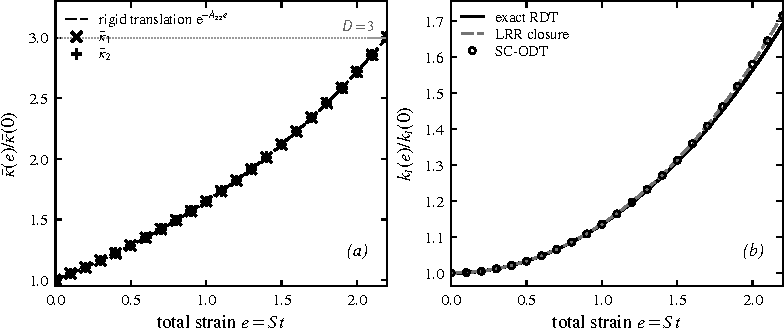
\includegraphics[width=\textwidth]{Figures/fig_cmk_rdt.pdf}
  \caption{Rapid-distortion limit (eddy events suppressed, inviscid)
  against the analytic reference of \citet{LeePiomelliReynolds1986}
  used by \citet{ChenMeneveauKatz2006}. (\textit{a}) Component
  spectral-centroid migration: the streamwise ($\times$) and upwash
  ($+$) centroids both follow the rigid-translation law and coincide
  throughout (the markers are interleaved so the two coincident series
  stay legible), reaching the deformation ratio $D=3$ at the end of the
  straining phase. (\textit{b}) Kinetic-energy amplification: the solver follows
  the closure trajectory, within $2\%$ of the exact rapid-distortion
  value at $e=2.20$.}
  \label{fig:s-cmk-rdt}
\end{figure}

With the eddy events and viscosity active, the full model (SC-ODT, C0.2) is no longer constrained to rigid translation, and the strain drives a measurable anisotropy between the components. Figure~\ref{fig:s-cmk-aniso} shows
the strain-induced migration of the streamwise and upwash component
centroids, each measured against the matched no-strain reference (the per-component form of the strain-on/strain-off construction, which
cancels the initialisation transient and the eddies' own relaxation):
the components diverge progressively under continued strain---the
streamwise migration reaching $1.9$ at the end of the straining phase
against $1.5$ for the upwash, both far below the rigid value $3$---so
the upwash component is held back most. This is the qualitative
behaviour CMK report---the strained spectrum departs from the
isotropic-translation expectation with the components responding
differently---and it is the spectral signature of the broadband
distortion analysed in the main text. The comparison is restricted to
its qualitative content, for three reasons stated plainly: the
band-limited initial spectrum differs from CMK's, so absolute levels
are not comparable; the line-resolved one-dimensional spectra and the
experiment's transverse/longitudinal projections are not the same
projection of the spectrum tensor; and the scale separation achieved
here ($\mathcal{L}/\eta\approx250$) is below the experimental
$\approx930$, whose compressed dissipation range exceeds feasible line
resolution. Within these limits the model reproduces the
rapid-distortion reference and the qualitative departure mechanism of
the benchmark; the quantitative spectral assessment is carried out in
the main text against the strained-box DNS, where the projection and
the initial spectrum are matched by construction. A direct numerical
simulation of the same straining--destraining cycle
\citep{GualtieriMeneveau2010}, at a Reynolds number below the
experiment's, reports the component variances and the pressure--strain
budget through the cycle and compares them with a Launder--Reece--Rodi
closure; it is the DNS counterpart against which the present model can
be set quantitatively on this configuration. A direct overlay is not
attempted here: their observable is the anisotropy through the full
straining--\emph{destraining} cycle, whereas the monotonic straining
phase reproduced above does not include the
strain reversal, so the comparison is kept at the level of the
independent confirmation their DNS provides for the experiment.

\begin{figure}
  \centering
  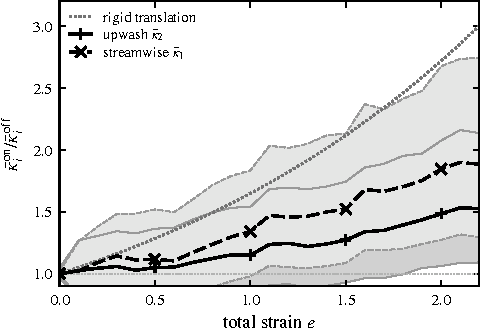
\includegraphics[width=0.62\textwidth]{Figures/fig_cmk_aniso.pdf}
  \caption{Full model (eddies and viscosity active; ensembles over
  $128$ realisations at $\nu=10^{-5}$): strain-induced migration of the
  streamwise and upwash component centroids, each as the geometric-mean ratio of the strained ensemble to the matched no-strain reference, against the rigid-translation law (grey dotted); the shaded bands span $\pm1$ geometric standard deviation of the ratio across the ensemble. The components diverge under
  strain---the upwash held back most---reproducing the qualitative
  departure-from-RDT mechanism of \citet{ChenMeneveauKatz2006}. The
  comparison is qualitative; see text.}
  \label{fig:s-cmk-aniso}
\end{figure}

% =========================================================================
\section{The intervention categories and variants}\label{sec:s-family}
% =========================================================================

Table~\ref{tab:s-interventions} records every intervention variant of the measured-limits campaign---its measured fine-scale effect on the transmission diagnostic and the remarks, keyed by the category.variant label---and figure~\ref{fig:s-klevels} shows the eddy-locked categories on all four diagnostic panels. The variant descriptions, together with the reference configurations C0.1 (standard ODT) and C0.2 (SC-ODT), are collected in Appendix~B of the main text. Each case was run at $1024$ realisations with seeds paired to SC-ODT (C0.2); effects are median paired same-seed contrasts, with ``significant'' meaning the $95\%$ bootstrap confidence interval excludes zero. The main text sets out the reading these results establish and retains the two figures that decide it (figures~15 and~16 of the main text: the relaxation clock and the five-way benchmark).
The case-by-case record follows.

Two categories fail for instructive reasons. Acceptance gating
(C1.1)---rejecting accepted eddies whose post-event state remains
anisotropic, at thresholds spanning $45$ to $98$ per cent
rejection---is scale-blind: at mild thresholds the surviving eddy
population reproduces the SC-ODT (C0.2) anisotropy budget in every
band (the gate self-selects eddies whose kernels were already going to
do the relaxing, and the unrelaxed field keeps generating candidates),
while at the harshest threshold the model merely drifts towards its
eddy-free limit. Restricting the gate to sub-band-scale eddies (C1.2)
sharpens the negative result: removing up to $97$ per cent of
small-eddy events leaves both the fine-scale anisotropy \emph{and} the
fine-scale energy unchanged, so no acceptance-gating scheme can
control transmission at this Reynolds number. Reweighting the
triplet-map images (C2.1; a middle image of relative size $\tfrac23$,
which halves the compression of the map's dominant central channel)
moves one-point and energy-containing
statistics---$\mathcal A_{\rm lo}$ falls significantly and the upwash
energy fraction with it---but not the fine scales: with the image
fractions summing to one, slowing the middle channel necessarily
speeds the outer ones, and one outer image maps the energy peak
directly into the measurement band.

What works is relaxation applied at the scale of the imbalance. After
each accepted eddy's map and kernels, the same energy-equalising
kernel procedure of the main text's formulation section is applied to
each of the three map images---the sub-interval's own triplet-map
displacement shape as the kernel, coefficients from the sub-interval's
own integrals, so that each sub-application conserves the momentum
components and the total kinetic energy exactly, with no map applied
and no random numbers drawn---and then recursively to $9$ and $27$
sub-regions. One sub-level (C3.1; $\ell/3$ for an eddy of size $\ell$)
is inconsequential: for the large eddies that feed the band, $\ell/3$
still sits above it. Two sub-levels (C3.2) produce the first
statistically significant fine-scale isotropisation among the
categories ($\mathcal A_{\rm hi}$ from $1.43$ to $1.27$ at $e=1$,
significant in both bands), and three sub-levels (C3.3) extend the
effect to deep strain: the sub-levels that work, $\ell/9$ and
$\ell/27$, are exactly those that reach the measured band. Band
energies move by only a few per cent throughout, the upwash energy
fraction and the intermittency tails are unchanged, and even at $e=0$,
before any strain, the fine-scale imbalance is pulled towards
component equality ($\mathcal A_{\rm hi}$ from $0.83$ to $0.95$).

Four further variants instantiate distinct candidate explanations for
the one remaining limitation, the fading of the gains beyond
$e\approx3$. Tying the recursion depth to the eddy size (C3.4;
subdividing while the sub-interval remains above a near-dissipative
floor, so that large eddies do proportionally more sub-scale work)
gives the gains of depth with no reversal at the deepest strain: both
bands significant at $e=1$ and the effect retaining its sign through
$e=3$. Iterating the two-level pass three times within each event
(C3.5) answers the amplitude hypothesis in the negative: a stronger
early isotropiser that overshoots at deep strain. Spatially
delocalising the relaxation---after each eddy, applying the kernel
isotropisation in $N$ randomly placed intervals of the same size,
overlaps allowed---tests whether the \emph{location} of the events is
the limiter: $N=1$ (C4.1) is inconsequential, and $N=3$ (C4.2) is
significant in both bands at $e=1$ but acts mainly at the
energy-containing scales, since the sampled intervals inherit the
eddy-size distribution and full-interval isotropisation acts at that
scale. Stacking the two ideas (C4.3)---the adaptive hierarchy inside
each sampled interval---is the strongest early isotropiser among the
categories ($\mathcal A_{\rm hi}$ from $1.43$ to $1.26$ at $e=1$) and
delivers the only significant deep-strain effect, in the
energy-containing band at $e=3.9$; yet at the fine scales and deep
strain it overshoots the depth-only variant significantly. For every
scheme locked to the eddy clock, depth sets where the relaxation acts
and is necessary; dosage and delocalisation raise the early gains in
proportion to the total relaxation delivered; and no eddy-locked
combination prevents the fine-scale fade beyond $e\approx3$.

\begin{table}
  \centering\small
  \begin{tabular}{p{0.07\textwidth}p{0.42\textwidth}p{0.40\textwidth}}
  label & fine-scale effect & remarks\\[2pt]
  \hline
  \multicolumn{3}{@{}l}{\emph{C1\quad acceptance gating}}\\[2pt]
  C1.1 & null at all thresholds; harshest drifts to eddy-free limit &
  gate is scale-blind: modulates eddy rate, not the scale allocation\\[4pt]
  C1.2 & null, including band \emph{energy} &
  fine scales are fed by large-eddy maps directly\\[2pt]
  \hline
  \multicolumn{3}{@{}l}{\emph{C2\quad map-image geometry}}\\[2pt]
  C2.1 & null (one-point statistics move: $\mathcal A_{\rm lo}$ $2.85\to2.50$ at
  $e=3.9$) & outer images feed the band in one step; channels trade off\\[2pt]
  \hline
  \multicolumn{3}{@{}l}{\emph{C3\quad sub-scale relaxation kernels (depth)}}\\[2pt]
  C3.1 & null within confidence intervals &
  $\ell/3$ sits above the measured band\\[4pt]
  C3.2 & $\mathcal A_{\rm hi}$: $1.43\to1.27$ at $e=1$ (significant, both bands) &
  first significant fine-scale isotropisation\\[4pt]
  C3.3 & significant at $e=1$ \emph{and} $e=3$ ($-12\%$ paired) &
  deepest levels reach the band\\[4pt]
  C3.4 & significant in both bands at $e=1$; no late-strain reversal &
  best of the categories: gains without the deep-strain overshoot\\[4pt]
  C3.5 & strongest at $e=1$ ($1.29$); overshoots at deep strain &
  per-event amplitude is not the limiter\\[2pt]
  \hline
  \multicolumn{3}{@{}l}{\emph{C4\quad concurrent relaxation}}\\[2pt]
  C4.1 & null & location alone is not the lever\\[4pt]
  C4.2 & significant in both bands at $e=1$, strongest at the energy-containing
  scales; fade persists & the sampled intervals act at eddy scale, so
  delocalising the events does not reach the fine scales\\[4pt]
  C4.3 & strongest early effect of the eddy-locked categories
  ($\mathcal A_{\rm hi}$ $1.43\to1.26$); low band significant even at $e=3.9$;
  fine scales overshoot depth-only at deep strain & dosage helps early and at
  large scales, and harms deep-strain fine scales wherever it is applied\\[2pt]
  \hline
  \multicolumn{3}{@{}l}{\emph{C5\quad independent relaxation clock}}\\[2pt]
  C5.1 & significant in both bands at \emph{every} strain, growing with
  strain---the fade broken---but the one-point anisotropy is suppressed
  ($u_2^2/2k_t$ $0.58\to0.41$ at $e=3.9$) & event-locked timing was the
  deep-strain limiter; a scale-blind event sequence fights the strain itself\\[4pt]
  \textbf{C5.2} & fine scales significant at every strain with no fade
  ($\mathcal A_{\rm hi}$ held at $1.30$--$1.44$); one-point trajectory intact for
  $e\lesssim2$, mildly reduced beyond & timing $+$ scale selectivity: the working
  form of the mechanism\\[4pt]
  C5.3 & fine scales significant at every strain, held below the
  matched-rate clock ($\mathcal A_{\rm hi}$ $1.15$--$1.40$); one-point
  anisotropy reduced further ($u_2^2/2k_t$ to $0.48$ at $e=3.9$ against
  SC-ODT's $0.58$) & the clock rate is a control: more relaxation holds
  the fine scales harder, at a proportionate one-point cost\\[2pt]
  \hline
  \end{tabular}
  \caption{The intervention categories on the transmission diagnostic, labelled by category.variant; variant descriptions and the reference configurations C0.1 (standard ODT) and C0.2 (SC-ODT) are in Appendix~B of the main text. Each case: $1024$ paired-seed realisations; effects are median paired same-seed contrasts, ``significant'' meaning the $95\%$ bootstrap confidence interval excludes zero. The size-capped clock \textbf{C5.2} (the clock-relaxed ODT of the main text), with C0.1 and C0.2, forms the five-way comparison.}
  \label{tab:s-interventions}
\end{table}

\begin{figure}
  \centering
  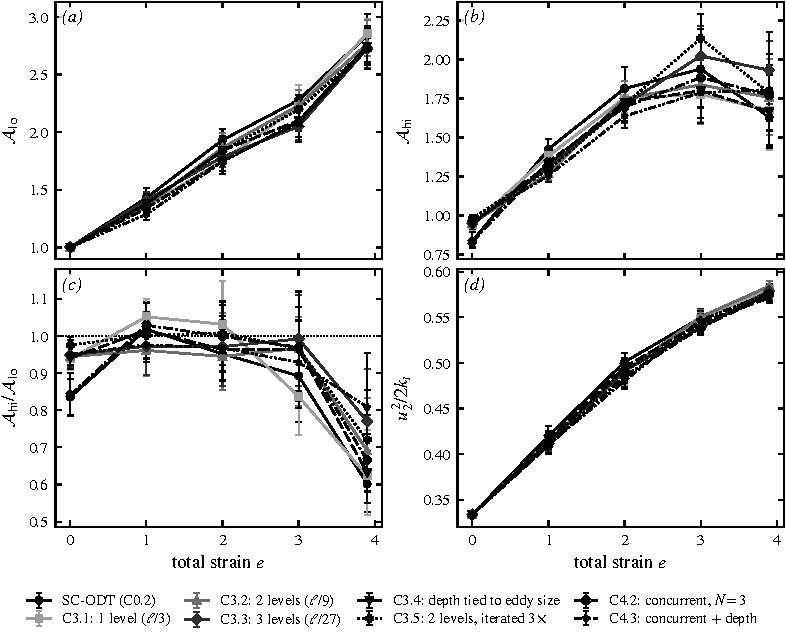
\includegraphics[width=\textwidth]{Figures/fig_klevels.pdf}
  \caption{Scale-local relaxation on the transmission diagnostic:
  (\textit{a}) energy-containing-band imbalance $\mathcal A_{\rm lo}$,
  (\textit{b}) fine-scale-band imbalance $\mathcal A_{\rm hi}$,
  (\textit{c}) transmission $\mathcal A_{\rm hi}/\mathcal A_{\rm lo}$,
  (\textit{d}) upwash energy fraction, against total strain: the SC-ODT reference (C0.2), sub-scale relaxation kernels at fixed depth (C3.1--C3.3), depth tied to eddy size (C3.4), the per-event iterated variant (C3.5), concurrent relaxation (C4.2, $N=3$ randomly placed same-size intervals per event), and the stacked variant (C4.3, concurrent intervals each running the adaptive hierarchy). Medians over $1024$ paired-seed realisations; error bars are the $95\%$ bootstrap confidence intervals of the median.}
  \label{fig:s-klevels}
\end{figure}

% =========================================================================
\section{The relaxation clock in the strained spectra}\label{sec:s-dividend}
% =========================================================================

Figure~\ref{fig:s-dividend} shows the spectral counterpart of the
transmission-diagnostic results of the main text, on the $1024$-realisation strained line spectrum ensembles at both rapidities (Appendix~B of the main text): the size-capped relaxation clock (C5.2) roughly halves the distance between the model's strained line spectra and the exact
rapid-distortion reference family, and---unlike SC-ODT (C0.2)---holds that distance \emph{constant in strain}. A frozen isotropic spectrum is included for reference; it stands for any calculation that feeds a frozen, undistorted inflow spectrum, which cannot represent the strained anisotropy at all, so its distance from the reference family grows to $45$--$51\%$ by $e=2$. The component-ratio
panel localises the improvement: exact rapid distortion drives the fine scales towards component equality, SC-ODT (C0.2) over-transmits the anisotropy there, and the clock (C5.2) moves the measured ratio towards the linear reference precisely below its size cap $\ell^*$.

\begin{figure}
  \centering
  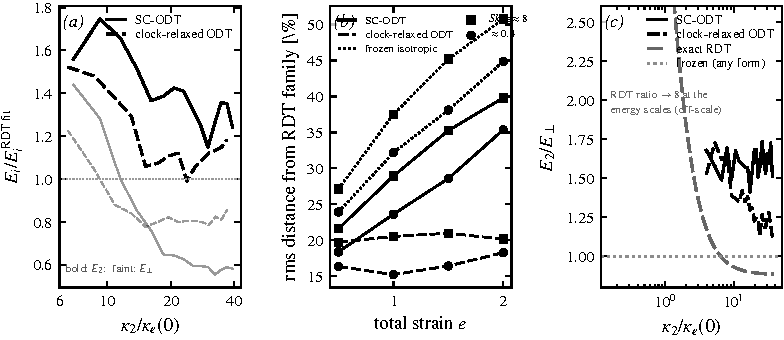
\includegraphics[width=\textwidth]{Figures/fig_dividend.pdf}
  \caption{(\textit{a}) Binned component spectra over their best
  exact-RDT-family curves at $e=2$, $Sk_t/\varepsilon\approx8$
  (solid: $E_2$; dashed: $E_\perp$): the SC-ODT (C0.2) misallocation (upwash high, transverse low) and its reduction by the clock (C5.2). (\textit{b}) rms log-distance from the exact-RDT family against total strain at both rapidities: frozen isotropic representation (gold), SC-ODT (C0.2, black), size-capped clock (C5.2, red); the clock's distance is strain-independent. (\textit{c}) Component ratio
  $E_2/E_\perp(\kappa_2)$ at $e=1$, rapid: measured SC-ODT (C0.2) and clock (C5.2) ensembles against the exact-RDT reference; any frozen form predicts the ratio $1$ identically.}
  \label{fig:s-dividend}
\end{figure}

% =========================================================================
\section{Operational steps of the leading-edge-noise chain}\label{sec:s-chain}
% =========================================================================

This section collects, in operational order, the steps of Part III of
the main text, from strained line ensembles to radiated level; every
step restates the main text.
\begin{enumerate}
\item \emph{Inflow representation.} For each total strain $e$ and
  strain-rate parameter, fit the exact-RDT-distorted von K\'arm\'an
  family to the median component line spectra of the
  $1024$-realisation ensemble---SC-ODT and, identically, the
  clock-relaxed variant---jointly in the upwash and transverse
  components, with the pre-distortion amplitude $A_0$ and energy
  wavenumber $\kappa_e$ the only free parameters. The rms log-residual
  of the fit is the distance envelope of the main text, carried
  through the chain as the input uncertainty.
\item \emph{Two-dimensional upwash spectrum.} Form
  $\Phi_{ww}(K_x,K_y;e)=A_0\int\Phi^{\rm RDT}_{22}
  (K_x,\kappa_2,K_y;e)\,\mathrm{d}\kappa_2$ by direct integration of
  the distorted components of the fitted family; the integration is
  verified against the wavevector-ensemble integrator of the main
  text (upwash-variance growth reproduced to under $1\%$).
\item \emph{Level and shape.} The noise kernel is linear in the
  upwash variance, so the variance ratio
  $\overline{u_2^2}(e)/\overline{u_2^2}(0)$ is taken from the
  measured line spectra and applied as the level; the fitted family
  supplies only the shape.
\item \emph{Geometry-free ratio.} Form
  $\mathcal K(K_x)=\pi\,\Phi_{ww}(K_x,0)^2\big/\!\int\Phi_{ww}
  (K_x,K_y)\,\mathrm{d}K_y$ for the distorted and for the frozen
  ($e=0$) input;
  $\Delta\mathrm{SPL}(K_x)=10\log_{10}
  [\mathcal K^{\rm distorted}/\mathcal K^{\rm frozen}]$, from which
  aerofoil geometry, response and observer cancel.
\item \emph{Absolute prediction.} At the reference configuration,
  physical units enter through two matching conditions only---the
  integral scale through $\kappa_e=0.7468/\mathcal{L}$ and the $e=0$
  upwash variance---and the far-field spectrum is assembled from the
  compact lift-dipole form of \citet{Amiet1975} with the exact Sears response \citep{Sears1941}; the frozen baseline is then the standard
  Amiet--von~K\'arm\'an prediction with no recalibration.
\item \emph{Validation chain.} Against the published measurements,
  all four inflows (frozen von K\'arm\'an, frozen Liepmann, SC-ODT,
  clock-relaxed ODT) pass through the identical non-compact response,
  with the Gershfeld thickness admittance applied to all four chains
  on the NACA0012 cases and the effective strain taken as the
  potential-flow stagnation-line accumulation truncated at the eddy
  scale.
\end{enumerate}

% =========================================================================
\section{Verification of the implementation}\label{sec:s-level1a}
% =========================================================================

The rapid-distortion checks of the main text verify the
\emph{formulation}; this section verifies the \emph{implementation},
in which the operator is not prescribed but reconstructed at every
substep: the line Reynolds stress is formed from the resolved field,
the closure supplies $\Pi^{(\mathrm r)}_{ij}$, the Lyapunov equation
of the main text is solved for $B_{ij}$, and
$\mathcal{A}_{ij}=-A_{ij}+B_{ij}$ is applied pointwise. To isolate
this chain the solver is run in the rapid-distortion limit---plane
strain, eddy events suppressed, zero molecular diffusion---from a
statistically isotropic resolved initial field, and the component
energies are evaluated as length-weighted line averages. With the
events inactive the line's component-energy evolution must coincide
with the closed moment equation across the whole strain range, not
merely at onset.

Figure~\ref{fig:s-level1a} shows that it does: the solver output lies
on the LRR trajectory over $0\le e\le4$ to within $10^{-4}$ in each
component fraction, so the per-substep stress reconstruction, Lyapunov
solve and operator assembly are correct at every state of anisotropy.
The comparison must be read correctly: the solver reproduces the
\emph{closure}, and it should---with the events and diffusion
suppressed the line carries no information beyond the single-point
statistics the closure itself uses. The offset from the exact solution
is the single-point closure error quantified in the main text's
finite-strain comparison, not an implementation error; agreement with
the exact solution here would indicate a fault. The fractions test
only the anisotropy; the kinetic energy, which the traceless rapid
term cannot change directly and which grows through the production
integral $\mathrm{d}\ln k_t/\mathrm{d}e=f_{22}-f_{11}$, provides the
independent magnitude check, and the solver reproduces the LRR
amplification to within $0.3\%$. The test requires a resolved spectral
initialisation (a white-noise start places energy at the grid scale,
where mesh-adaption interpolation damps it) and a strain-resolved
timestep bound in the inviscid limit; both effects act nearly
isotropically, so the energy panel is what distinguishes them.

\begin{figure}
  \centering
  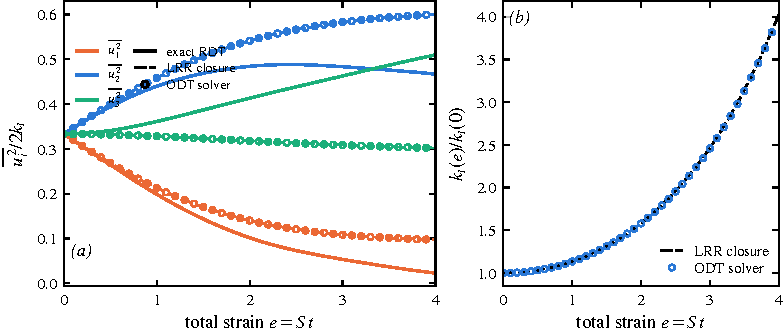
\includegraphics[width=\textwidth]{Figures/fig_level1a.pdf}
  \caption{Verification of the SC-ODT implementation under plane
  strain, eddy events suppressed and zero molecular diffusion.
  (\textit{a}) Component energy fractions; (\textit{b}) kinetic-energy
  amplification $k_t(e)/k_t(0)$. Open symbols: the SC-ODT line solver
  (length-weighted line averages), by component
  ($\circ\,\overline{u_1^2}$, $\square\,\overline{u_2^2}$,
  $\triangle\,\overline{u_3^2}$); dashed: the LRR closure integrated as
  a moment equation; solid with filled symbols: exact rapid-distortion
  theory. The solver reproduces the closure to $10^{-4}$ in the
  fractions and $0.3\%$ in the energy; the offset from the exact
  solution is the closure error quantified in the main text, as it
  must be.}
  \label{fig:s-level1a}
\end{figure}

% =========================================================================
\section{The strained ODT line}\label{sec:s-line}
% =========================================================================

Figure~\ref{fig:s-line} is a space--time view of a single realisation of
the line under the three model variants of the main text, advanced from
identical initial fields (matched seed and spectral initial condition, so
the three differ only by the model). Standard ODT (strain off) keeps its
full width; SC-ODT and clock-relaxed ODT compress under the plane strain,
the physical line half-width (black envelope) falling by a factor of
about seven over $e=0$--$4$. The upwash velocity is normalised at each
instant so the eddy structure stays visible as the fluctuations decay;
amplitudes are therefore not comparable across strain, only the structure
and the geometric compression. The clock-relaxed strip retains finer
structure at high strain than SC-ODT---the single-realisation signature
of the fine-scale hold that the $1024$-realisation statistics of
\S\,\ref{sec:s-dividend} quantify.

\begin{figure}
  \centering
  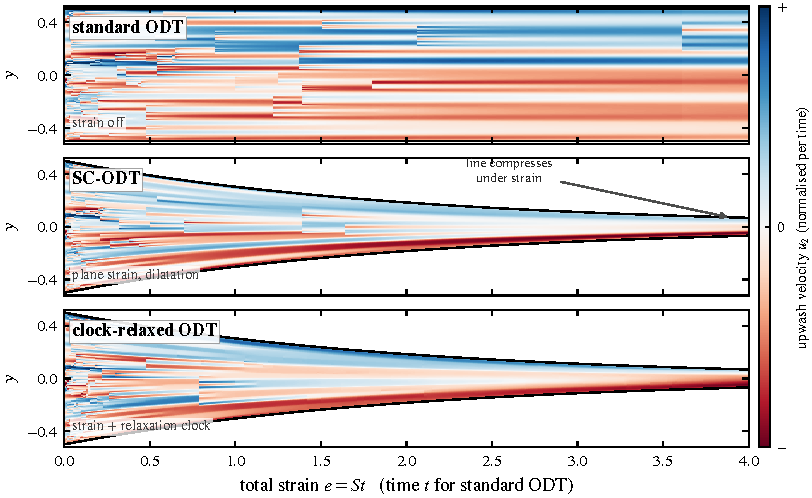
\includegraphics[width=\textwidth]{Figures/fig_hero_lines_color.pdf}
  \caption{Space--time evolution of the ODT line, upwash velocity $u_2$
  (normalised at each instant; blue positive, red negative, colour
  intensity the magnitude), for standard ODT, SC-ODT and clock-relaxed
  ODT, advanced from matched initial fields. Time runs left to right as the total strain $e=St$
  (elapsed time for the unstrained standard-ODT case); the black envelope
  is the physical line half-width. Standard ODT keeps its full width;
  SC-ODT and clock-relaxed ODT compress under the plane strain, the
  clock-relaxed line retaining finer structure at high strain.}
  \label{fig:s-line}
\end{figure}

The difference between SC-ODT and the clock-relaxed model is not
apparent in a single realisation of the velocity itself---the two
diverge into distinct realisations---but it shows in the small-scale
\emph{structure}. Figure~\ref{fig:s-line-zoom} isolates it: the
high-pass (small-scale) upwash field over the high-strain window
$e=2.5$--$4$, in the stretched coordinate $y/\text{half-width}$ so the
compressed line fills the frame. SC-ODT smooths to a few coarse bands as
the fine scales relax away, whereas the clock-relaxed line stays
grainy---its sub-scale relaxation events keep fine-scale structure alive,
the single-realisation counterpart of the sustained fine-scale imbalance
seen in the ensemble statistics of \S\,\ref{sec:s-dividend}.

\begin{figure}
  \centering
  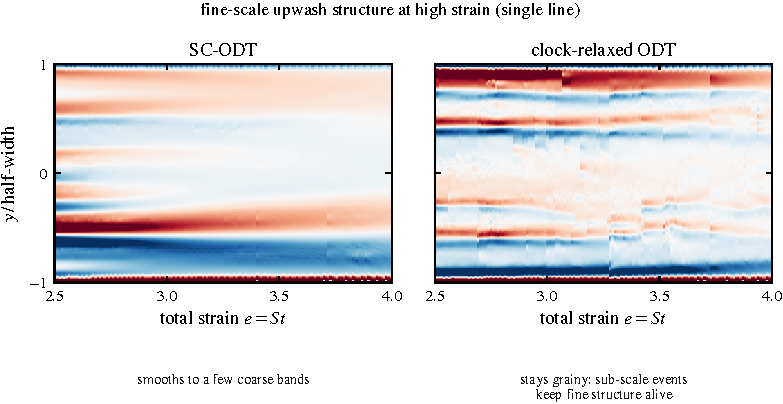
\includegraphics[width=\textwidth]{Figures/fig_hero_diff_contour.pdf}
  \caption{Small-scale (high-pass) upwash structure of a single ODT line
  in the high-strain window, $e=2.5$--$4$, in the stretched coordinate
  $y/\text{half-width}$: SC-ODT (left) against clock-relaxed ODT (right);
  blue positive, red negative, colour intensity the magnitude.
  SC-ODT smooths to a few coarse bands; the clock-relaxed line stays
  grainy, its sub-scale relaxation events sustaining fine-scale structure
  (the vertical striations are individual events). Amplitudes are
  normalised and the two are different realisations, so the contrast is
  the clock's structural signature, not a pointwise difference.}
  \label{fig:s-line-zoom}
\end{figure}

\bibliographystyle{jfm}
\bibliography{jfm}

\end{document}
